\documentclass[11pt]{article}

\usepackage[english]{babel}         % American English
\usepackage[T1]{fontenc}            % Required for hyphenation
\usepackage[utf8]{inputenc}         % UTF-8 encoding

\usepackage{amssymb,amsmath,amsthm} % AMS
\usepackage{url}                    % Typesetting URLs
\usepackage{hyphenat}               % Hyphenation with \hyp
\usepackage[scaled=0.8]{beramono}   % Nice bold/italic teletype font
\usepackage{float}                  % Tuning placement of figures
\usepackage{graphicx}               % Inclusion of graphics
\usepackage{caption,subfig}         % Subfigures
\usepackage{xspace}                 % Proper spacing after macros
\usepackage{alltt}                  % Verbatim with macros
%\captionsetup[subfloat]{justification=raggedleft}
\usepackage[colorlinks=true,citecolor=black,linkcolor=black,urlcolor=blue]{hyperref}

\bibliographystyle{plain}  % TEMPORARY
%\usepackage{etoolbox}
%\apptocmd{\thebibliography}{\raggedright}{}{} % No Underfull \hbox

% New commands
%
\newcommand{\nb}[1]{\marginpar{{\color{red}\small #1}}}
\newcommand{\XML}{\textsf{XML}\xspace}
\newcommand\fig{\textsc{Figure}}

\title{The Average Height of Catalan Trees\\
  by Counting Lattice Paths}
\author{Nachum Dershowitz \and Christian Rinderknecht}
\date{}

\begin{document}

\maketitle

\hfill \emph{In memoriam} Philippe Flajolet, friend and colleague

\bigskip

Structured documents, like books, articles and web pages, are composed
of chapters, sections, paragraphs, figures, annexes, indexes etc., the
occurrences of which being mutually constrained, for instance, it is
understood that a section must belong to a chapter, and annexes are
located at the end of a document. This hierarchical layout is meant to
facilitate reading, and it supports the search of specific pieces of
information. When considering computer systems, these data must be
uniformly encoded with a formal language. For instance, an email
contains at least the sender's address, a subject or title, the
recipient's address and a body of plain text: these elements
correspond to \emph{nodes} in a structure called a \emph{Catalan
  tree}, a.k.a.\@ ordered trees or rooted plane trees. The email
\begin{alltt}
From: Me
Subject: Homeworks
To: You

  A \textbf{deadline} is a due date for a \emph{homework}.
\end{alltt}
can be modeled by the tree in \fig~\ref{fig:mail},
\begin{figure}
\centering
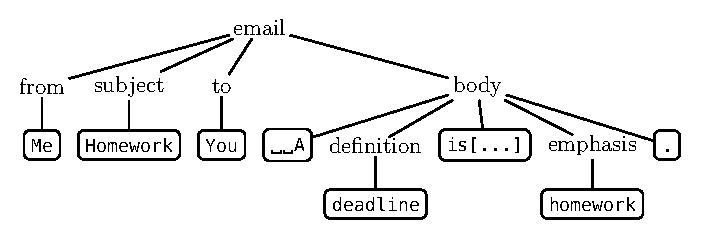
\includegraphics[bb=71 620 389 723]{mail}
\caption{An email viewed as a Catalan tree\label{fig:mail}}
\end{figure}
where the topmost node (`email') is called the \emph{root} and the
framed pieces of text are \emph{leaves} --~computer scientists grow
trees upside down. The inner nodes hold \emph{metadata}, or markup,
that is, information about the data contained in the subtree.

Catalan trees are a pervasive data structure in computer science, in
that they are a natural representation for hierarchical data. For
example, in \XML (eXtensible Markup Language), information is stored
in text nodes at the leaves, and, consequently, its retrieval requires
the traversal of the tree from the root to a leaf. The \emph{height}
of a tree is the number of nodes on a maximal, simple path from the
root to a leaf; for example, follow down the nodes depicted
as~\(\circ\) in the tree of height~\(5\) in \fig~\ref{fig:catalan}.
\begin{figure}
\centering
\includegraphics{catalan}
\caption{Catalan tree of height~\(5\).\label{fig:catalan}}
\end{figure}

In general, the maximum cost of a search is proportional to the height
of the tree, and the determination of the average height becomes
relevant when performing a series of random
searches~\cite{VitterFlajolet:1990}. The mathematical study of this
average quantity often relies on advanced analytical tools, and the
purpose of the present note is to propose a partial simplification of
these approaches by using combinatorics.

\section*{The Analytical Derivation}

Let~\(h_n\) be the average height of Catalan trees with \(n\)~edges
and \(H_{n,h}\) the number of Catalan trees with \(n\)~edges and
height~\(h\). We then have \(h_n = S_n/C_{n}\), where \(S_n := \sum_{h
  \geqslant 1} h \cdot H_{n,h}\) and~\(C_n\) is the number of Catalan
trees with~\(n\) edges.

To gain a purchase on the sum~\(S_n\), we might define~\(A_{n,h}\) as
being the number of trees with \(n\)~edges and height less than or
equal to~\(h\). Of course, we have \(A_{n,h} = A_{n,n+1} = C_{n}\), if
\(h > n\). Then \(H_{n,h} = A_{n,h}-A_{n,h-1}\). Formulas can be
further simplified by letting~\(B_{n,h}\) be the number of trees with
\(n\)~edges with height greater than~\(h\):
\begin{equation}
S_n = \sum_{h \geqslant 1}h(A_{n,h}-A_{n,h-1})
    = \sum_{h \geqslant 1}h(B_{n,h-1}-B_{n,h}) = \sum_{h\geqslant 0} B_{n,h}.
\label{eq:Sn}
\end{equation} 
Knuth, de Bruijn, and Rice~\cite{KnuthdeBruijnRice:1972} published a
landmark paper in~\oldstylenums{1972}, where they obtained the
asymptotic approximation of the average height~\(h_n\). They started
by modeling the problem with a generating function~\cite{Wilf:1990}
that satisfies a recurrence equation whose solution expresses the
generating function in terms of continued fractions of Fibonacci
polynomials. Integration over complex numbers is utilized to obtain
the formula
\begin{equation}
B_{n,h-1} = \sum_{k \geqslant 1}\left[\binom{2n}{n+1-kh}
           - 2\binom{2n}{n-kh} + \binom{2n}{n-1-kh}\right].
\label{eq:Bn}
\end{equation}
The authors conclude by employing real and complex analysis to obtain
asymptotic expansions of~\(B_{n,h}\), \(S_n\), and~\(h_n\). The main
term is \(h_n \sim \sqrt{\pi n}\), where \(f(n) \sim g(n)\) means
\(\lim_{n \rightarrow \infty} f(n)/g(n) = 1\), wherever
\(f\)~and~\(g\) are defined.
  
The purpose of the present note is to show how to circumvent heavy
analytic techniques in the derivation of
equation~\eqref{eq:Bn}. Instead, we propose an elementary
combinatorial proof based on the enumeration of the Dyck paths of a
certain height, which are in bijection with Catalan trees of a related
height. We find this bijective proof to be more intuitive, in
particular to computer scientists, for whom the result matters for the
analysis of algorithms. Technically, our approach is in tune with
Mohanty~\cite{Mohanty:1979}, as well as Dershowitz and
Zaks~\cite{DershowitzZaks:1981}.

\section*{Counting Catalan trees}

Before we determine~\(B_{n,h}\), let us solve a related and easier
question: finding the number~\(C_n\) of Catalan trees with~\(n\)
edges, called the Catalan number.

In \oldstylenums{1984}, Kemp~\cite[p.~64]{Kemp:1984} (see also
\cite{FlajoletNebelProdinger:2006}) derived equation~\eqref{eq:Bn} by
analytical means too, but, instead of working directly with Catalan
trees, he used certain lattice paths in an integer grid. The
\emph{monotonic lattice paths}~\cite{Mohanty:1979,Humphreys:2010} are
made up of two kinds of steps oriented upwards and rightwards,
starting at \((0,0)\) with an upward step. \emph{Dyck paths} of
length~\(2n\) are monotonic paths ending at \((n,n)\) that never
venture below the diagonal; an example with \(n=6\) is shown in
\fig~\ref{fig:dyck}.
\begin{figure}
\centering
\subfloat[Dyck path of length 12.\label{fig:dyck}]{%
\includegraphics[bb=62 634 165 721]{dyck}
}
\qquad\qquad
\subfloat[Catalan tree with 6 edges.\label{fig:tree}]{%
\includegraphics[bb=60 663 138 721,scale=1.5]{tree}
}
\caption{Bijection between Dyck paths and Catalan trees.\label{fig:bijection}}
\end{figure}

\paragraph{A bijection with Dyck paths}

Crucially, there is a bijection between Dyck paths of length~\(2n\)
and Catalan trees with \(n\)~edges~\cite{Klarner}.

This bijection is shown on an example in \fig~\ref{fig:bijection}. To
construct the lattice path in \fig~\ref{fig:dyck} from the tree in
\fig~\ref{fig:tree}, we imagine that the tree is a roadmap and our
avatar plans a tour starting at the root as follows: we take the
rightmost unvisited road (from the avatar's viewpoint), else we
backtrack: in the end, we have taken each road twice: there, and back
again. More technically, in \fig~\ref{fig:dfs},
\begin{figure}
\centering
\includegraphics[scale=1.2]{dfs}
\caption{Preorder traversal \label{fig:dfs}}
\end{figure}
we follow the dotted arrows: each downward arrow in the tree
corresponds to a step up~\(\uparrow\) (called a \emph{rise}) in the
lattice, and an upward arrow in the tree to a step
right~\(\rightarrow\) (called a \emph{fall}). In the tree, the series
is \(\downarrow\) \(\downarrow\) \(\uparrow\) \(\downarrow\)
\(\downarrow\) \(\uparrow\) \(\uparrow\) \(\uparrow\) \(\downarrow\)
\(\uparrow\) \(\downarrow\) \(\uparrow\), which becomes \(\uparrow\)
\(\uparrow\) \(\rightarrow\) \(\uparrow\) \(\uparrow\) \(\rightarrow\)
\(\rightarrow\) \(\rightarrow\) \(\uparrow\) \(\rightarrow\)
\(\uparrow\) \(\rightarrow\) in the lattice. If we follow the latter
from the start at the bottom left corner \((0,0)\), we obtain the path
in \fig~\ref{fig:dyck}. This kind of traversal is called
\emph{preorder} or document order, because it is the way we would read
the document represented by the tree, from cover to cover. Note as
well that there are~\(n+1\) nodes if, and only if, there are~\(n\)
edges in the tree, because there is one edge per node going up, save
for the topmost node (\emph{root}).

\paragraph{The inclusion-exclusion principle}

The previous bijection allows us to count the Catalan trees with
\(n\)~edges by counting instead the Dyck paths of length~\(2n\). 

It is easy to count all the monotonic paths of length~\(2n\) because
there are as many as choices of \(n\)~rises amongst \(2n\)~steps, that
is, \(\binom{2n}{n}\). To count only the Dyck paths, we need to
subtract the number of paths that start with a rise and cross the
diagonal.

This approach is an instance of the method known as the
\emph{inclusion\hyp{}exclusion principle}, whereby a direct and
difficult enumeration of a set is replaced by the easier enumeration
of a strict superset and the subtraction of the cardinal of a strict
subset (so that the resulting sets are equal).

An example of a path which is not a Dyck path is shown in
\fig~\ref{fig:reflection},
\begin{figure}[b]
\centering
\includegraphics[scale=0.9]{reflection}
\caption{Reflection of a prefix with respect to \(y = x - 1\).\label{fig:reflection}}
\end{figure}
drawn in bold. The first point reached below the diagonal is used to
plot a dotted line parallel to the diagonal. All the steps from that
point back to \((0,0)\) are then changed into their counterpart: a
rise is replaced by a fall and vice-versa. The resulting segment is
drawn as a dashed line. This operation is called a
\emph{reflection}~\cite{Renault:2008}. The crux of the matter is that
we can reflect each monotonic path crossing the diagonal into a
distinct path from \((1,-1)\) to \((n,n)\). These reflected paths can,
in turn, be reflected when they reach the dotted line back into their
original counterpart. In other words, the mapping is
bijective. (Another intuitive and visual approach to the same result
has been published by Callan~\cite{Callan_1995}.) Consequently, there
are as many monotonic paths from \((0,0)\) to \((n,n)\) that cross the
diagonal as there are monotonic paths from \((1,-1)\) to
\((n,n)\). The latter are readily enumerated: \(\binom{2n}{n-1}\). In
conclusion, the number of Dyck paths of length~\(2n\) is
\begin{align*}
C_n &= \binom{2n}{n} - \binom{2n}{n-1}
= \binom{2n}{n} - \frac{(2n)!}{(n-1)!(n+1)!}\\
&= \binom{2n}{n} - \frac{n}{n+1} \cdot \frac{(2n)!}{n!n!}
 = \binom{2n}{n} - \frac{n}{n+1} \binom{2n}{n} = \frac{1}{n+1}\binom{2n}{n}.
\end{align*}
Using Stirling's formula for the asymptotic equivalence, we draw:
\begin{equation}
C_n = \frac{1}{n+1}\binom{2n}{n} \sim \frac{4^n}{n\sqrt{\pi n}},
      \quad\text{as \(n \rightarrow \infty\)}.
\label{eq:Cn}
\end{equation}

In~\oldstylenums{1996}, Sedgewick and
Flajolet~\cite{SedgewickFlajolet:1996,FlajoletSedgewick:2009} derived
the enumerations of Catalan trees by height, also using analytic
combinatorics, but they employed real analysis to obtain the
asymptotic approximation of~\(B_{n,h}\). They
write~\cite[p.~260]{SedgewickFlajolet:1996}:
\begin{quote}
\it This analysis is the hardest nut that we are cracking in this
book. It combines techniques for solving linear recurrences and
continued fractions, generating function expansions, especially by the
Lagrange inversion theorem, and binomial approximations and
Euler\--Maclaurin summations.
\end{quote}

\section*{A Combinatorial Proof}

To avoid the aforementioned advanced techniques used to derive
equation~\eqref{eq:Bn}, we use again a bijection between Dyck paths
and Catalan trees, but, this time, the key point is that Catalan trees
with~\(n\) edges and height~\(h\) are in bijection with Dyck paths of
length~\(2n\) and height \(h-1\). This simple observation allows us to
reason on the height of the Dyck paths and transfer our findings back
to Catalan trees.

With the determination of~\(A_{n,h}\) in mind, let us consider a Dyck
path of length \(2n\) and height~\(h-1\), as in \fig~\ref{fig:height}.
\begin{figure}[!b]
\centering
\subfloat[Dyck path of length \(2n\) and
height \(h-1\).\label{fig:height}]{
\includegraphics[bb=66 565 252 724,scale=0.9]{height}}
\qquad
\subfloat[Path from \(A\) to \(\Omega\) avoiding the boundaries
  \(y=x+s\) and \(y=x-t\).\label{fig:mohanty}]{
\includegraphics[scale=0.9]{mohanty}}
\caption{Paths avoiding diagonal boundaries.\label{fig:boundaries}}
\end{figure}
The double lines are boundaries that may not be attained by the
path. This is in fact a special case of a general monotonic path
between two diagonal boundaries, as shown in \fig~\ref{fig:mohanty},
where \(s\)~denotes the vertical distance from~\(A\), and \(t\),~the
horizontal distance from~\(A\). It is well known that the number of
monotonic paths from~\(A(0,0)\) to~\(\Omega(a,b)\) avoiding the
boundaries \(y = x + s\) and \(y = x - t\) is
\begin{equation}
\left\lvert\mathcal{L}(a,b;t,s)\right\rvert = \sum_{k \in \mathbb{Z}}\left[\binom{a+b}{b+k(s+t)} - \binom{a+b}{b+k(s+t)+t}\right].
\label{eq:mohanty}
\end{equation}
The proof by Mohanty~\cite[p.~6]{Mohanty:1979} of this formula is
based on the reflection principle and the principle of inclusion and
exclusion, which we used earlier. We quote his proof here verbatim,
because it is rarely found in print nowadays.
\begin{proof}[Proof {\rm (Mohanty~\cite{Mohanty:1979})}]
 For brevity, call the boundaries \(x=y+t\) and
  \(x=y-s\), \(\mathcal{L}^{+}\) and \(\mathcal{L}^{-}\),
  respectively. Denote by~\(A_1\) the set of paths that reach
  \(\mathcal{L}^{+}\), by~\(A_2\) the set of paths that reach
  \(\mathcal{L}^{+}\), \(\mathcal{L}^{-}\) in that order, and in
  general by~\(A_i\) the set of paths reaching \(\mathcal{L}^{+}\),
  \(\mathcal{L}^{-}\), \(\mathcal{L}^{+}\), \ldots\@ (\(i\)~times) in
  the specified order. Similarly, let~\(B_i\) be the set of paths
  reaching \(\mathcal{L}^{-}\), \(\mathcal{L}^{+}\),
  \(\mathcal{L}^{-}\), \ldots\@ (\(i\)~times) in the specified order. An
  application of the usual method of inclusion and exclusion yields
\begin{equation}
\left\lvert\mathcal{L}(a,b;t,s)\right\rvert = \binom{a+b}{b} + \sum_{i
\leqslant 1}(-1)^{i}(\lvert{A_i}\rvert + \lvert{B_i}\rvert),
\label{eq:L}
\end{equation}
where~\(\lvert{A_i}\rvert\) and~\(\lvert{B_i}\rvert\) are evaluated by
using the reflection principle repeatedly. For example,
consider~\(A_3\). Since every path in~\(A_3\) must
reach~\(\mathcal{L}^{+}\), \(A_3\) when reflected about
\(\mathcal{L}^{+}\) becomes the set of paths from \((t,-t)\) to
\((a,b)\) each of which reaches~\(\mathcal{L}^{+}\) after reaching
\(\mathcal{L}^{-}\). Another reflection about \(\mathcal{L}^{-}\)
would make~\(A_3\) equivalent to the set of paths from \((-s-t,s+t)\)
to \((a,b)\) that reach~\(\mathcal{L}^{+}\), which in turn can be
written as \(R(a+s+t,b-s-t; 2s+3t)\). [Note: \(R(a,b;t)\) is the set
  of paths from \((0,0)\) to \((a,b)\) reflected
  about~\(\mathcal{L}^{+}\).] Thus, since \(\lvert{R(a,b;t)}\rvert =
\binom{a+b}{a-t}\), we have
\begin{equation*}
\left\lvert{A_3}\right\rvert = \binom{a+b}{a-s-2t},
\end{equation*}
and, more generally,
\begin{equation*}
\left\lvert{A_{2j}}\right\rvert = \binom{a+b}{a+j(s+t)}
\quad\text{and}\quad
\left\lvert{A_{2j+1}}\right\rvert = \binom{a+b}{a-j(s+t)-t}.
\end{equation*}
The expressions for \(\lvert{B_{2j}}\rvert\),
\(\lvert{B_{2j+1}}\rvert\), \(j=0, 1, 2, \dots\), with
\(\lvert{A_0}\rvert\), \(\lvert{B_0}\rvert\) being \(\binom{a+b}{b}\),
are obtained by interchanging \(a\)~with~\(b\) and
\(s\)~with~\(t\). Substitution of these values in~\eqref{eq:L}
yields~\eqref{eq:mohanty} after some simplifications.
\end{proof}

Resuming our argument, if we match the figures in
\fig~\ref{fig:boundaries}, we find \(s=h\), \(t=1\), \(a=b=n\),
hence \(a+b=2n\) and \(b+k(s+t)=n+k(h+1)\),
which we plug into formula~\eqref{eq:mohanty} and change \(h\)~into \(h-1\):
\begin{equation*}
A_{n,h-1} = \sum_{k \in \mathbb{Z}}\left[\binom{2n}{n+kh} -
           \binom{2n}{n+1+kh}\right].
\end{equation*}
After splitting the sum into \(k<0\), \(k=0\), and \(k>0\), then
changing the sign of~\(k\) in the first case, using \(\binom{p}{q} =
\binom{p}{p-q}\) in the second, and lastly gathering the remaining
sums ranging over \(k \geqslant 1\), we reach
\begin{align*}
A_{n,h-1}
  &= - \sum_{k \geqslant 1}\left[\binom{2n}{n+1-kh} -
    2\binom{2n}{n-kh} + \binom{2n}{n-1-kh}\right]\\
  &\phantom{=}\; + \binom{2n}{n} - \binom{2n}{n-1}.
\end{align*}
Recognising \(C_n\), we simplify as follows:
\begin{equation*}
C_n - A_{n,h-1}
  = \sum_{k \geqslant 1}\left[\binom{2n}{n+1-kh} -
    2\binom{2n}{n-kh} + \binom{2n}{n-1-kh}\right].
\end{equation*}
Finally, recalling that \(B_{n,h} = A_{n,n+1} - A_{n,h}\) and \(C_n =
A_{n,n+1}\), we arrive at
\begin{equation*}
B_{n,h-1} = \sum_{k \geqslant 1}
            \left[\binom{2n}{n+1-kh} - 2\binom{2n}{n-kh}
            + \binom{2n}{n-1-kh}\right],
\end{equation*}
which is none other than our target, equation~\eqref{eq:Bn}.

In this way, we have achieved our goal merely by enumerating lattice
paths, and hopefully have, in the process, made this classic result
less daunting.

\section*{Asymptotics}

We could stop here, but we would like to give a hint as to how the
asymptotic approximation is carried out. Equation~\eqref{eq:Sn}
entails \(S_{n} = \sum_{h \geqslant 1}B_{n,h-1}\); therefore
\begin{equation*}
S_{n} = \sum_{k' \geqslant 1}d(k') %\cdot
        \left[\binom{2n}{n+1-k'} - 2\binom{2n}{n-k'}
        + \binom{2n}{n-1-k'}\right],
\end{equation*}
where~\(d(k')\) is the number of positive divisors of~\(k'\), but
complex analysis is
needed~\cite{KnuthdeBruijnRice:1972,FlajoletGourdonDumas:1995}. Another way is to express the binomials in terms of \(\binom{2n}{n-kh}\):
\begin{align*}
\binom{2n}{n-m+1} &= \frac{(2n)!}{(n-m+1)!\,(n+m-1)!}\\
                  &= \frac{(2n)!\,(n+m)}{(n-m)!\,(n-m+1)(n+m)!} 
                   = \frac{n+m}{n-m+1}\binom{2n}{n-m},\\
\binom{2n}{n-m-1} &= \frac{(2n)!}{(n-m-1)!\,(n+m+1)!}\\
                  &= \frac{(2n)!\,(n-m)}{(n-m)!\,(n+m)!\,(n+m+1)}
                   = \frac{n-m}{n+m+1}\binom{2n}{n-m}.
\end{align*}
Therefore,
\begin{equation*}
\binom{2n}{n-m+1} - 2\binom{2n}{n-m} + \binom{2n}{n-m-1}
= 2 \cdot \frac{2m^2-(n+1)}{(n+1)^2-m^2}\binom{2n}{n-m}.
\end{equation*}
Let \(F_n(m) = (2m^2-n)/(n^2-m^2)\). We have
\begin{equation*}
S_{n} = 2 \cdot \sum_{h \geqslant 1}\sum_{k \geqslant 1} F_{n+1}(kh)
\cdot \binom{2n}{n-kh}.
\end{equation*}
From equation~\eqref{eq:Cn} and \(h_n = S_n/C_n\), we deduce \(h_{n} =
(n+1)S_{n}{\binom{2n}{n}}^{-1}\), hence we must approximate
\((n+1)F_{n+1}(m)\) and \(\binom{2n}{n-m}\binom{2n}{n}^{-1}\). On the
one hand, we have
\begin{equation*}
F_{n+1}(m) \sim \frac{2m^2-n}{n^2} \sim \frac{2m^2-n}{n(n+1)},
\end{equation*}
so \((n+1)F_{n+1}(kh) \sim 2k^2h^2\!/n-1\). On the other hand,
Sedgewick and Flajolet~\cite[4.6, 4.8]{SedgewickFlajolet:1996} show
\begin{equation*}
\binom{2n}{n-m}{\binom{2n}{n}}^{-1} \sim e^{-m^2\!/n}.
\end{equation*}
Assuming that the tails (the implicit error terms) of the two previous
approximations decrease exponentially, we have
\begin{equation*}
h_{n} \sim \sum_{h \geqslant 1}\sum_{k \geqslant 1}
(4k^2h^2\!/n - 2)e^{-k^2h^2\!/n}
= \sum_{h \geqslant 1}H(h/\!\sqrt{n}), 
\end{equation*}
where \(H(x) = \sum_{k \geqslant 1}(4k^2x^2-2)e^{-k^2x^2}\). Finally,
Sedgewick and Flajolet~\cite[\S 5.9]{SedgewickFlajolet:1996}, on the one
hand, and Graham, Knuth, and
Patashnik~\cite[\S 9.6]{GrahamKnuthPatashnik:1994}, on the other hand,
use real analysis to conclude
\begin{equation*}
h_n \sim \sum_{h \geqslant 1}H(h/\!\sqrt{n})
    \sim \sqrt{n} \int_0^{\infty}H(x) dx \sim \sqrt{\pi n}.
\end{equation*}
The end of this derivation is difficult because the error terms in the
bivariate asymptotic approximations must be carefully checked, so it
is unlikely to be simplified further. 

Remarkably, the main term $\sqrt{\pi n}$ in the asymptotic value for
height can also be obtained by simple lattice-path
arguments~\cite{DershowitzZaks:1990}.

\bibliography{lattice}
%%-*-latex-*-

\paragraph{Summary}

The average height of Catalan trees of a given size is a structural
parameter important in the analysis of algorithms, as it measures the
expected maximum cost of a search in a tree. This parameter has been
studied first with generating functions and complex variable theory,
yielding an asymptotic approximation. Later on, real analysis was used
instead of complex analysis. We have further reduced the conceptual
difficulty by replacing generating functions with the enumeration of
monotonic lattice paths, whose graphical representations make the
derivation much more intuitive.

%% \noindent\textbf{Keywords:} Catalan tree; ordered tree; planted plane
%% tree; expected height; lattice path enumeration; Dyck path;
%% average-case analysis of algorithms
%\end{abstract}


\end{document}
